\chapter{FEniCS}

The \fenics project started in 2003 and the aim was create software that automates a finite element discretisation and solution of differential equations. The core libraries used within \fenics are DOLFIN \cite{LoggWells2010a,LoggWellsEtAl2012a}, FFC \cite{KirbyLogg2006a,LoggOlgaardEtAl2012a,OlgaardWells2010b}, FIAT \cite{Kirby2012a,Kirby2004a}, Instant, UFC \cite{AlnaesLoggEtAl2009a,AlnaesLoggEtAl2012a} and UFL \cite{AlnaesEtAl2012,Alnaes2012a}. Along the these core packages \fenics has a few extra optional packages that can be found here \url{http://fenicsproject.org/applications/}.

\section{Overview}

One of the key ideas of \fenics was to be able to write an easy to use software package for the solution of partial differential equations (PDEs). The main underlying code base for \fenics is written in C++. and Python


\fenics supports large range of a different finite element function space. Thus allowing \fenics to be used from electromagnetic problems to fluid. The full list of support elements can be found in table~\ref{tab:FunctionSpace}.
\begin{table}[h!]
    \begin{center}
        \begin{tabular}{ l  l }
            Name    &Usage\\
            \hline
            Argyris*    &``ARG''\\
            Arnold-Winther* &``AW''\\
            Brezzi-Douglas-Fortin-Marini*   &``BDFM''\\
            Brezzi-Douglas-Marini   &``BDM''\\
            Bubble  &``B''\\
            Crouzeix-Raviart    &``CR''\\
            Discontinuous Lagrange  &``DG''\\
            Hermite*    &``HER''\\
            Lagrange    &``CG''\\
            Mardal-Tai-Winther* &``MTW''\\
            Morley* &``MOR''\\
            Nedelec 1st kind H(curl)    &``N1curl''\\
            Nedelec 2nd kind H(curl)    &``N2curl''\\
            Quadrature  &``Q''\\
            Raviart-Thomas  &``RT''
        \end{tabular}
        \caption{Avaliable finite element function space (*only partly supported)}
        \label{tab:FunctionSpace}
    \end{center}
\end{table}



This breath introduction to \fenics will go through how to set up a very simple test case, namely the Poisson equation. For this simple problem we will consider both Dirichlet and Neumann boundary conditions and show how to set up the PDE in its variational form.


\section{Poisson example}

For a simple example to see how FEniCS works consider the Poisson equation. Defining $\Omega \subset \R^n$ to be the domain and the boundary as $\partial \Omega = \Gamma_D \cup \Gamma_N$ where $\Gamma_D$ and $\Gamma_N$ correspond to the Dirichlet and Neumann boundaries respectively. Thus, the Poisson equation with corresponding boundary conditions reads as:
\begin{equation} \label{eq:poisson}
 \left. \begin{aligned}
-\Delta u &= f \quad \mbox{in } \Omega\\
 u &= 0 \quad \mbox{in } \Gamma_D\\
\nabla u \cdot n &= g \quad \mbox{in } \Gamma_N
    \end{aligned}
 \right.
 \qquad \text{}
\end{equation}
For this example we will be considering the following function, domains and boundaries to be:
\begin{itemize}
\item $f = (x-\nicefrac{1}{2})^2-4(y-\nicefrac{1}{2})^4$
\item $g = 5x$
\item $\Omega = [0,1]\times[0,1]$
\item $\Gamma_D = \{(0,y) \cup (1,y) \quad | \quad  0\leq y\leq 1\}$
\item $\Gamma_N = \{(x,0) \cup (x,1) \quad | \quad  0\leq x\leq 1\}$
\end{itemize}
Defining the following trial and test function spaces  $\mathcal{V}$ and $\bar{\mathcal{V}}$ as
\begin{equation} \label{eq:PoissonFuncSpace}
 \left. \begin{aligned}
    \mathcal{V}&=H^1_{u_0}(\Omega)=\left\{\,{u}\in H^1(\Omega)\,:\,\text{${u}=u_{0}$ on $\partial\Omega$}\,\right\}, \\
    \bar{\mathcal{V}}&=H^1_0(\Omega)=\left\{\,{u}\in H^1(\Omega)\,:\,\text{${u}={0}$ on $\partial\Omega$}\,\right\}.
 \end{aligned}
 \right.
 \qquad \text{}
\end{equation}
Thus the variational formulation of (\ref{eq:poisson}) depends on finding $u \in \mathcal{V}$ such that
\begin{equation}
\label{eq:PoissonWeak}a(u,v) = L(v) \quad \forall v\in\bar{\mathcal{V}},
\end{equation}
where
\begin{equation}
a(u,v) = \int_{\Omega} \nabla u \cdot \nabla v \, dx \quad \mbox{and} \quad L(v) = \int_{\Omega} fv dx +\int_{\Gamma_N}gv\,ds.
\end{equation}

\subsection{Defining mesh and function space}

For this example we want to consider a uniform unit square mesh. This is created by using the following python code
\begin{pythoncode}
mesh = UnitSquareMesh(32,32)
\end{pythoncode}
Once the mesh is create we no turn to the function space. For this model problem we want to consider the function space $\mathcal{V}$  and $\bar{\mathcal{V}}$ defined by \eqref{eq:PoissonFuncSpace}. Therefore, the discrete finite element space use is the following space
$$\uu{V}_h  = \{\, \uu{u}\in H_1( \Omega)\, :\, \uu{u}|_K \in {\mathcal P}_{1}(K), \, K \in{\mathcal T}_h \, \},$$
where ${\mathcal T}_h=\{K\}$ regular and quasi-uniform triangles. This function space is create in \fenics using the following command
\begin{pythoncode}
V = FunctionSpace(mesh,'CG',1)
\end{pythoncode}

\subsection{Defining subdomains}
Separating different parts of the boundary is easily done within FEniCS. For this our simple Possion model the boundary is split up into two parts. The top and bottom defines the Dirichlet boundary condition whilst the left and right portions of the boundary define the Neumann conditions. Before partitioning the domain into the Dirichlet and Neumann boundaries we need to define the different sections of the boundary. This is done using classes as follows:
\begin{pythoncode}
# Defining boundary classes
class Left(SubDomain):
    def inside(self, x, on_boundary):
        return near(x[0], 0.0)

class Right(SubDomain):
    def inside(self, x, on_boundary):
        return near(x[0], 1.0)

class Bottom(SubDomain):
    def inside(self, x, on_boundary):
        return near(x[1], 0.0)

class Top(SubDomain):
    def inside(self, x, on_boundary):
        return near(x[1], 1.0)

# Initialize sub-domain instances
left = Left()
top = Top()
right = Right()
bottom = Bottom()
\end{pythoncode}
Using the classes above we group the Dirichlet and Neumann boundaries together. These can then be used to set up the boundary conditions for our problem.
\begin{pythoncode}
boundaries = FacetFunction("size_t", mesh)
boundaries.set_all(0)
left.mark(boundaries, 1)
right.mark(boundaries, 1)
top.mark(boundaries, 2)
bottom.mark(boundaries, 2)
\end{pythoncode}

\subsection{Boundary Conditions and weak formulation}

The boundaries have been split into their separate domains so now we can think about defining the boundary conditions, bilinear and linear (\ref{eq:PoissonWeak}) forms.

First consider the homogeneous Dirichlet boundary:
$$  u = 0 \quad \mbox{in } \Gamma_D.$$
The Dirichlet boundary condition is created by using the  \code{DirichletBC} class. When defining Dirichlet boundary conditions on separate subdomains we need to use four inputs to the  \code{DirichletBC} class. The first one is the function space that the boundary condition applies to, the value on the boundary and then the last two arguments define which part of the boundary the boundary condition is defined on.
\begin{pythoncode}
u0 = Constant(0.0)
bc = DirichletBC(V, u0, boundaries,1)
\end{pythoncode}

To define the variational form of the problem we first need to determine the trial function  \code{u} and test function  \code{v} belonging to the function space $\mathcal{V}$. Furthermore, the source term $f$ and Neumann condition $g$ are required in the linear form $L(v)$. Both are defined using the  \code{Expression} class. Together with the trial and test functions the variational form can be created using the following code:
\begin{pythoncode}
# Define variational problem
u = TrialFunction(V)
v = TestFunction(V)
f = Expression("(pow(x[0]-0.5,2)-4*pow(x[1]-0.5,4))")
g = Expression("(5*x[0])")
a = inner(grad(u), grad(v))*dx
L = f*v*dx + g*v*ds(2)
\end{pythoncode}


\subsection{Assembly and solving}

Now the variational  (or weak form) have been stated the next step is to solve the problem. This can be done in two was within FEniCS
\begin{itemize}
    \item[1.] Assemble system and solve
    \item[2.] Solve without assembly.
\end{itemize}
First, consider assembling then solve the system. This can be done by using the {\code{assemble\_system}} class. This class takes the variational form as the inputs and the Dirichlet boundary condition.
\begin{pythoncode}
A, b = assemble_system(a,L,bc)
\end{pythoncode}
The final solving step is the same for both ways. To do this we first define a function {\code{u}} in the corresponding function space ($\mathcal{V}$) that will represent the solution. Next, calling the \code{solve} function with either the matrix \code{A} and vector \code{b} as the arguments or the variational form will compute the solution using sparse direct solvers which is the  default solving method for \fenics
\begin{pythoncode}
u = Function(V)
solve(A,u.vector(),b)
solve(a == L, u, bc)
\end{pythoncode}

\subsubsection{Optional solution parameters}

For simplicity above the \code{solve} used \fenics default parameters. However, this may not necessarily be the most efficient so may want to change these parameters. It is well known for example that multigrid is the most efficient solve for the Poisson problem. Here is how to set this up.
\begin{pythoncode}
solve(a == L, u, bc,
            solver_parameters=dict(linear_solver="cg",
            preconditioner="amg"))
\end{pythoncode}
For more optional parameters use the following commands:
\begin{pythoncode}
print list_krylov_solver_methods()
print list_krylov_solver_preconditioners()
print list_linear_algebra_backends()
print list_linear_solver_methods()
print list_lu_solver_methods()
\end{pythoncode}

Instead of using FEniCS's inbuilt solving function you can use other external packages. For instance you can link you your FEniCS code with Trilinos \cite{Trilinos-Users-Guide,Trilinos-Overview}, PETSc \cite{petsc-web-page,petsc-user-ref} or your own code.

\subsection{Visualisation}

Once you have solved your problem the next step is to either visualise or save the result. To output the solution in a VTK file you need to create a file with \code{.pvd} suffix. This enables you to use external software (for example ParaView \cite{}) to visualise the solution. Alternatively FEniCS's has an interface for the VTK visualisation tools. We do this by using the \code{plot} command.
\begin{pythoncode}
# Save solution in VTK format
file = File("poisson.pvd")
file << u

# Plot solution
plot(u, interactive=True)
\end{pythoncode}

\begin{figure}[h!]
  \centering
    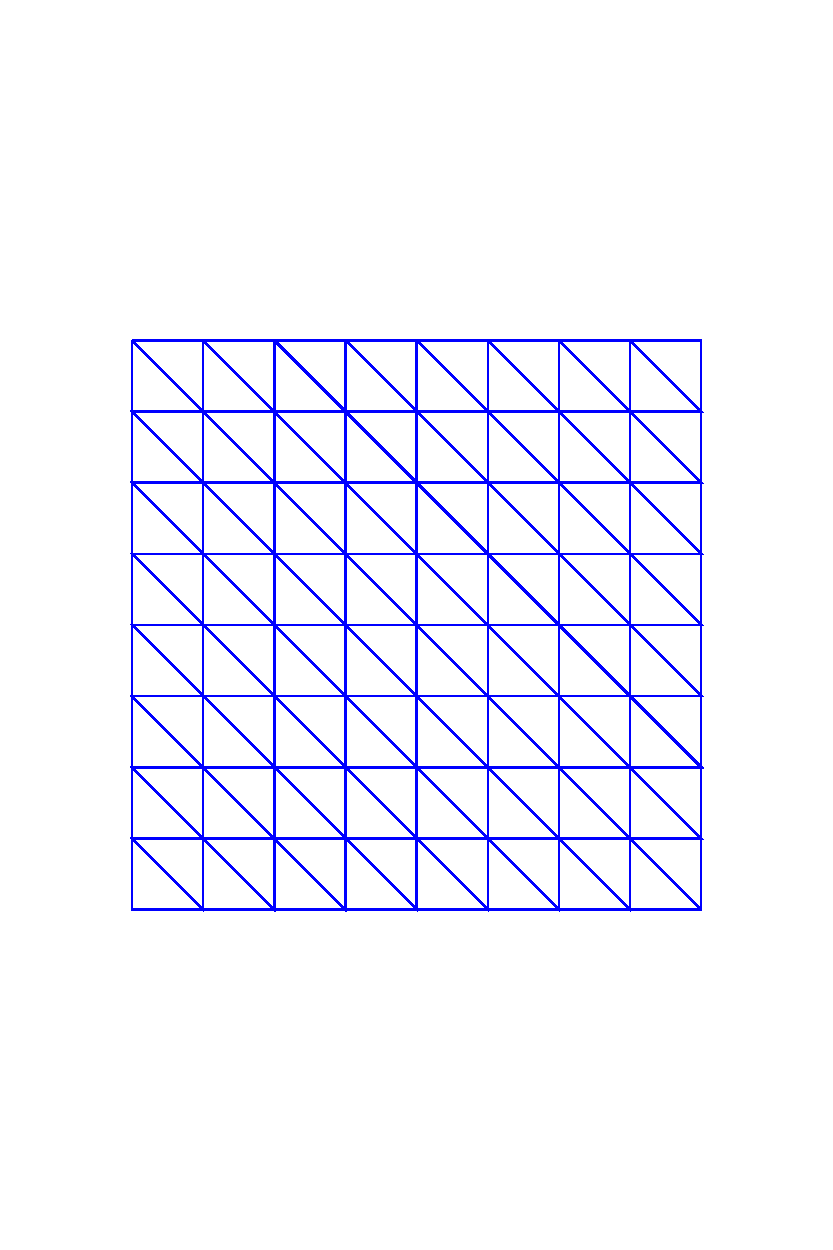
\includegraphics[scale=.6]{../FEniCS/Figures/dolfin_plot_1}
\caption{Numerical solution to (\ref{eq:poisson})}
\end{figure}


% \bibliographystyle{plain}
% \bibliography{/home/mwathen/Dropbox/MastersResearch/MHD/THESIS/ref/ref}

